%%%%%%%%%%%%%%%%%%%%%%%%%%%%%%%%%%%%%%%%%
% Facial Expresion Recognition with Convolutional Neural Networks
% 
% Lewe Ohlsen
% Fachhochschule Wedel
%
% Latex Template by Frits Wenneker (http://www.howtotex.com)
%
%%%%%%%%%%%%%%%%%%%%%%%%%%%%%%%%%%%%%%%%%

%----------------------------------------------------------------------------------------
%	PACKAGES AND OTHER DOCUMENT CONFIGURATIONS
%----------------------------------------------------------------------------------------

\documentclass[twoside]{article}

\usepackage{lipsum} % Package to generate dummy text throughout this template
\usepackage{graphicx} % Figures from matplotlib
\graphicspath{ {figures/} }

\usepackage[sc]{mathpazo} % Use the Palatino font
\usepackage[T1]{fontenc} % Use 8-bit encoding that has 256 glyphs
\linespread{1.05} % Line spacing - Palatino needs more space between lines
\usepackage{microtype} % Slightly tweak font spacing for aesthetics

\usepackage[hmarginratio=1:1,top=32mm,columnsep=20pt]{geometry} % Document margins
\usepackage{multicol} % Used for the two-column layout of the document
\usepackage[hang, small,labelfont=bf,up,textfont=it,up]{caption} % Custom captions under/above floats in tables or figures

\usepackage{booktabs} % Horizontal rules in tables
\usepackage{float} % Required for tables and figures in the multi-column environment - they need to be placed in specific locations with the [H] (e.g. \begin{table}[H])
\usepackage{hyperref} % For hyperlinks in the PDF

\usepackage{lettrine} % The lettrine is the first enlarged letter at the beginning of the text
\usepackage{paralist} % Used for the compactitem environment which makes bullet points with less space between them

\usepackage{abstract} % Allows abstract customization
\renewcommand{\abstractnamefont}{\normalfont\bfseries} % Set the "Abstract" text to bold
\renewcommand{\abstracttextfont}{\normalfont\small\itshape} % Set the abstract itself to small italic text

\usepackage{titlesec} % Allows customization of titles
\usepackage[utf8]{inputenc}
\renewcommand\thesection{\Roman{section}} % Roman numerals for the sections
\renewcommand\thesubsection{\Roman{subsection}} % Roman numerals for subsections
\titleformat{\section}[block]{\large\scshape\centering}{\thesection.}{1em}{} % Change the look of the section titles
\titleformat{\subsection}[block]{\large}{\thesubsection.}{1em}{} % Change the look of the section titles


%----------------------------------------------------------------------------------------
%	TITLE SECTION
%----------------------------------------------------------------------------------------

\title{\vspace{-15mm}\fontsize{16pt}{10pt}\selectfont\textbf{Facial Expression Recognition with\\ Convolutional Neural Networks}} % Article title 

\author{
	\large
	\textsc{Lewe Ohlsen}\\[2mm] % Your name
	\normalsize Fachhochschule Wedel \\ % Your institution
	\normalsize \href{mailto:minf101062@fh-wedel.de}{minf101062@fh-wedel.de} % Your email address
	\vspace{-5mm}
}
\date{}

%----------------------------------------------------------------------------------------

\begin{document}

\maketitle % Insert title

%----------------------------------------------------------------------------------------
%	ABSTRACT
%----------------------------------------------------------------------------------------

\begin{abstract}

\noindent El barómetro es un instrumento de medición atmosérica, específicamente utilizado en la determinación de la fuerza por unidad de superficie ejercida por el peso de la atmósfera. Existe un gran número de equipos atmoféricos con distintos tipos de estos aparátos y son diariamente utilizados ya que la presión atmosférica juega un papel importante en la determinación y pronóstico del tiempo así como en el área de investigación al momento de realizarse experimentos ya que pueden llegar a afectar o hacer variar el funcionamiento de muchos aparatos electrónicos y mecánicos.

\end{abstract}

%----------------------------------------------------------------------------------------
%	ARTICLE CONTENTS
%----------------------------------------------------------------------------------------

\begin{multicols}{2} % Two-column layout throughout the main article text

\section{Introduction}

Automatically recognizing facial expressions is an interesting and challenging problem in many fields, including human computer interaction (HCI) and artificial emotional intelligence. The projects goal is to build a device to process live webcam images, detect faces and classify the emotion of each face.

As Convolutional Neural Networks (CNNs) have proven to be successful with many kinds of image classification  problems, I will focus on building a classifier using a state of the art CNN implementation.

%------------------------------------------------

\section{Datasets}

Paul Ekmans 1969 research paper "Facial Expressions" elaborates that facial expressions can be interpreted as emotions. He suggests that there are six classes of basic emotion that can be found across all human cultures: anger, disgust, fear, happiness, sadness, and surprise. In this project, these classes are used as emotion classes for predictions.

For training an artificial neural network to classify facial expressions to these basic emotions, a dataset with labeled images of faces is required.

\subsection{FER-2013}
The FER-2013 Dataset consists of roughly 37.000 images showing faces of people expressing a certain emotion. Images are 48x48 pixel grayscale images of faces. These images have been centered automatically to show a similar region of the face in every sample. 

Initially, the dataset is split into two subsets: A training set that is used to fit the prediction and a test set to evaluate the prediction results.


\begin{figure}[H]
	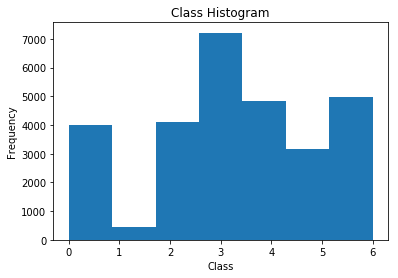
\includegraphics[width=0.48\textwidth]{class_dist}
	\caption{Class distribution across the training dataset}
\end{figure}

\subsection{Cohn-Kanade}



%------------------------------------------------

\section{Discussion and Conclusion}



%----------------------------------------------------------------------------------------
%	REFERENCE LIST
%----------------------------------------------------------------------------------------

\begin{thebibliography}{99} % Bibliography - this is intentionally simple in this template

\bibitem[http://fluidos.eia.edu.co/]{Figueredo:2009dg}

\newblock {\em Fluidos, Carlos Toro s.}

\bibitem[http://www.windows2universe.org/]{Figueredo:2009dg}

\newblock {\em Becca Hatheway}

\bibitem[http://meteorologia.pucp.edu.pe/]{Figueredo:2009dg}

\newblock {\em Hernan Castillo, Pedro Ríos}

\bibitem[http://www.ammonit.com/Manuales]{Figueredo:2009dg}

\newblock {\em Ammonit Measurement GmbH}

 
\end{thebibliography}

%----------------------------------------------------------------------------------------

\end{multicols}

\end{document}
